\documentclass[12pt]{article}

\delimitershortfall-1sp
\newcommand\abs[1]{\left|#1\right|}

\usepackage{amsmath}
\usepackage{mathtools}
\usepackage{authblk}

\title{Linear DNA CXS simulation}
\author{Shenglan Qiao}
\begin{document}
\maketitle

I present here some simulated CXS signal for a system of water and a linear DNA double-helix with 17 bps. Figure~\ref{fig:dna} shows the system; it consists of  3919 water molecules surrounding the linear DNA. To sample different configurations of water molecules around the DNA, I run MD simulations with the DNA fixed in space while the water molecules are allowed to interact with and move around it. In this way, I sample a total of 20,000 DNA-water configurations. To compute the scattering intensity from a single DNA-water system, each one of the 20,000 configurations is rotated to a randomly sampled orientation. 

\begin{figure}[h!]
\center
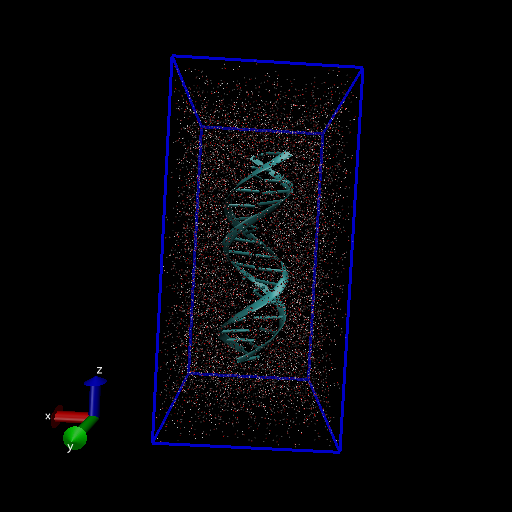
\includegraphics[width=0.4\textwidth]{figures/dna_box.png}
\caption{MD simulation box: system contains linear DNA with 17 bps and 3919 water molecules; size of the simulation box (outlined in blue) is 3.960 by 4.058 by 8.082 nm.}
\label{fig:dna}
\end{figure}

The total scattering intensity from such 20,000 exposures is shown in Figure~\ref{fig:scatter} ($q = 0.7 \sim 2.2 \AA^{-1}$). We ignore scattering from hydrogen atoms. The intensity profile as a function of momentum transfer indicates a well known water peak at $\sim 2.0 \AA^{-1}$. The water peaks tend to be board (see Figure S3 in \cite{waterSellberg} for an example). Therefore the sharp peaks in the intensity profile must have come from structures in the DNA.



\begin{figure}[h!]
\center
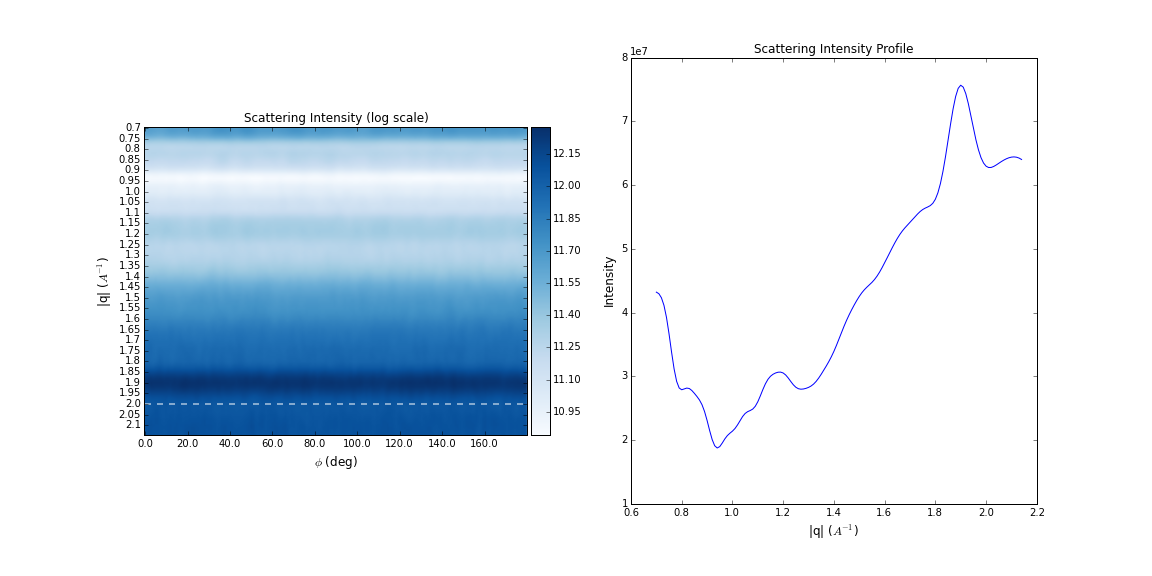
\includegraphics[width=1.1\textwidth]{figures/Iscat.png}
\caption{Total scattering intensity and profile of 20,000 orientations of single DNA systems. The color scale is a log scale in order to increase contrast. The white dotted lines indicate maximum momentum transfer for bulk water at $\sim 2.0 \AA^{-1}$. In the intensity profile, the water peak centered around $\sim 2.0 \AA^{-1}$ should be much boarder than the DNA peaks; the peak at $\sim 1.9 \AA^{-1}$, for instance, must have come from the DNA.}
\label{fig:scatter}
\end{figure}

From individual scattering intensities, I compute the autocorrelator at different momentum transfers (Figure~\ref{fig:autocorr}). Most of the variations in structures concentrate in the $q = 0.7 \sim 0.9 \AA^{-1}$ and $q = 1.85  \sim 1.97 \AA^{-1}$ regions. 

\begin{figure}[h!]
\center
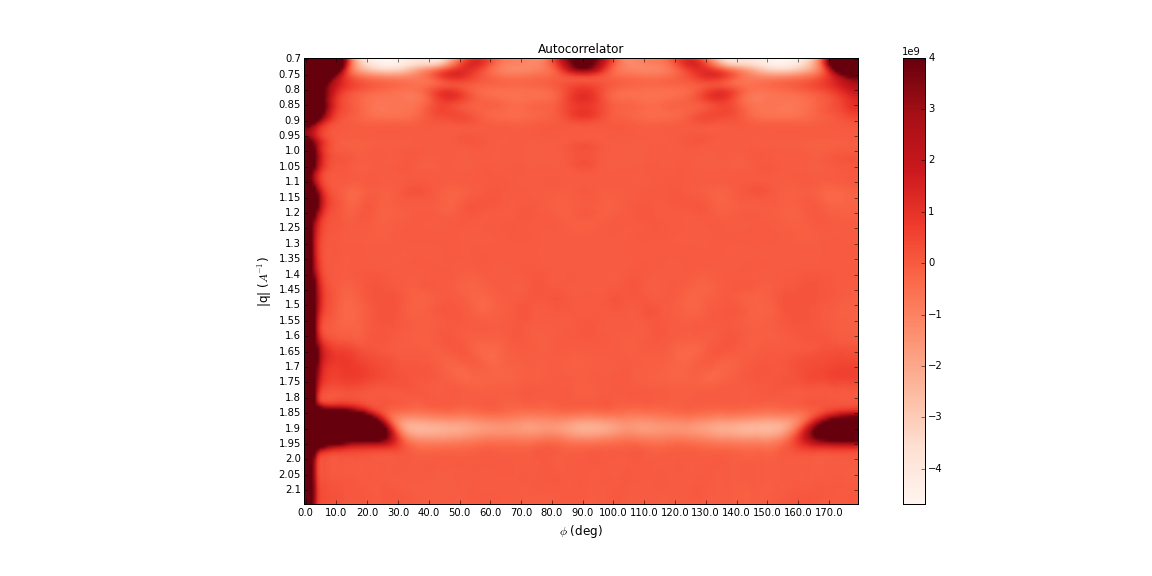
\includegraphics[width=1.1\textwidth]{figures/autocorr.png}
\caption{Autocorrelation, computed from 20,000 individual scattering intensities, each containing a single DNA system with a different orientation. }
\label{fig:autocorr}
\end{figure}

Projecting the autocorrelator at each momentum transfer to even-order Legendre polynomials and plotting the coefficients, we can see that at different length scales different kinds of symmetry dominate. Figure~\ref{fig:LProj} shows the zeroth through eighth even-ordered projections and Figure~\ref{fig:LPs} gives a sense of what each polynomial looks like. The x-axis of Figure~\ref{fig:LProj} has been converted to length in $\AA$. Figure~\ref{fig:LProj} shows two regions with lots of "wiggles" in the autocorrelator and a relatively flat region in the middle. The shorter length scale region is between about 3 $\AA$ to 3.5 $\AA$; this is approximately the distance between the two planes formed by consecutive basepairs. This makes sense to me because there should be a lot of correlation between position of atoms between two consecutive base pairs. The longer length scale region with lots of "wiggles" starts around 7 $\AA$.  My best guess is that starting at around 7.0 $\AA$, we begin to see correlations between atoms that are on the two different single strands of the double helix (the double helix has a radius of approximately 10 $\AA$). 

The purpose of doing this simulation is to inform our data analysis effort. I offer a few takeaways: 1) we should look for strong signals from the linear DNA in the $q > 0.7 \AA^{-1}$ region where scattering from water is weaker and $q = 1.85  \sim 1.97 \AA^{-1}$ region where short range correlation between atoms in the DNA is strong. 2) We can potentially use the well-known water intensity profile to calibrate a gain map for the detector (this can be dangerous because the gain map will have only radial dependence but no angular dependence). 3) We should do simulations for even smaller angles (what is the smallest $q$ in our data?) and also run simulations for supercoiled DNA.

\begin{figure}[h]
\center
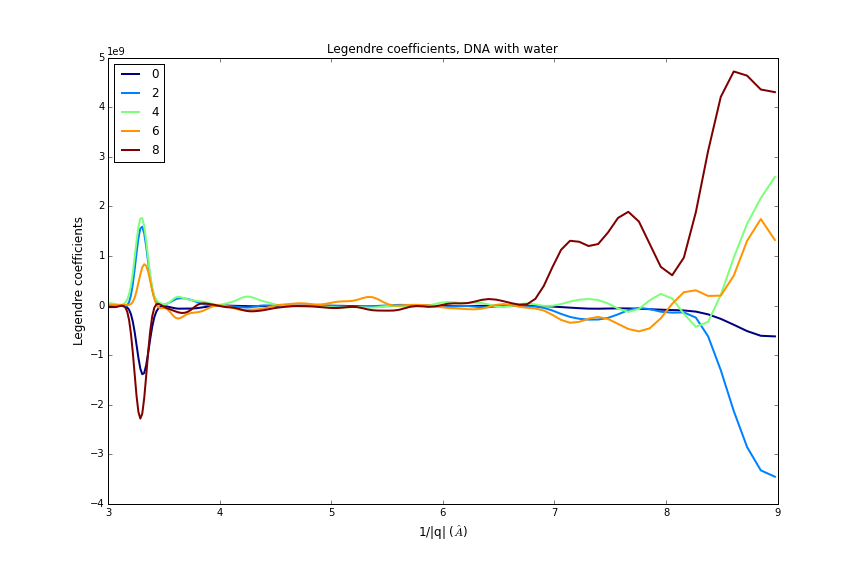
\includegraphics[width=0.8\textwidth]{figures/LProj_real.png}
\caption{Legendre projections of autocorrelators into the zeroth to eighth even-order Legendre polynomials. }
\label{fig:LProj}
\end{figure}

\begin{figure}[h]
\center
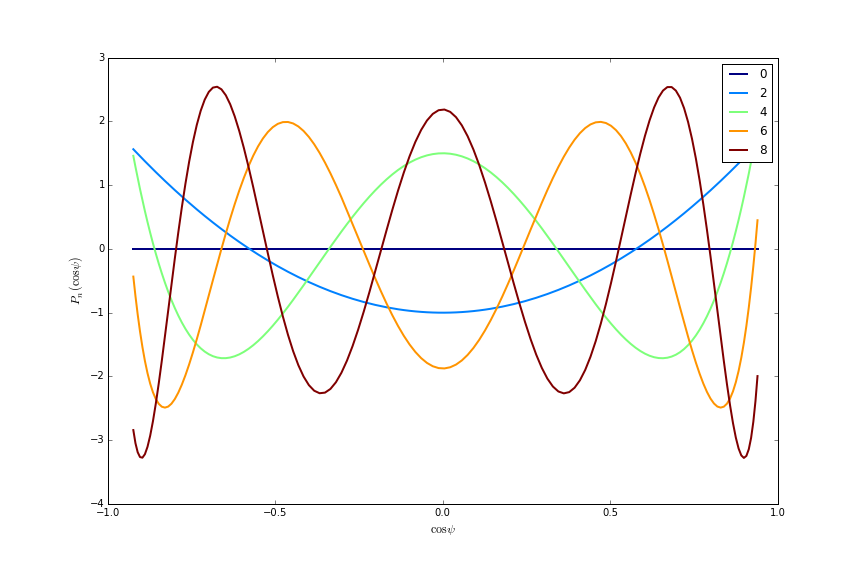
\includegraphics[width=0.8\textwidth]{figures/LPs_8.png}
\caption{The zeroth to eighth even-order Legendre polynomials. }
\label{fig:LPs}
\end{figure}


\begin{thebibliography}{9}
\bibitem{waterSellberg}
Sellberg, JA et. al.
\textit{Ultrafast X-ray probing of water structure below the homogeneous ice nucleation.}
Nature 510, 381?384 (19 June 2014)
\end{thebibliography}
\end{document}